\documentclass[final]{siamltex}
\usepackage{psfig}
\usepackage{algorithmic}
\usepackage{graphicx}
\usepackage{ipe}
%\usepackage[colorlinks=true, pdfstartview=FitV, linkcolor=blue,
%            citecolor=blue, urlcolor=blue]{hyperref}

\newcommand{\centeripe}[1]{\begin{center}\Ipe{#1}\end{center}}
\newcommand{\comment}[1]{}

\newcommand{\centerpsfig}[1]{\centerline{\psfig{#1}}}

\newcommand{\etal}{{\em et al\/}}
\newcommand{\adhoc}{{\em ad hoc\/}}

\newcommand{\seclabel}[1]{\label{sec:#1}}
\newcommand{\Secref}[1]{Section~\ref{sec:#1}}
\newcommand{\secref}[1]{\mbox{Section~\ref{sec:#1}}}

\newcommand{\applabel}[1]{\label{app:#1}}
\newcommand{\Appref}[1]{Appendix~\ref{app:#1}}
\newcommand{\appref}[1]{\mbox{Appendix~\ref{app:#1}}}

\newcommand{\tablabel}[1]{\label{tab:#1}}
\newcommand{\Tabref}[1]{Table~\ref{tab:#1}}
\newcommand{\tabref}[1]{Table~\ref{tab:#1}}

\newcommand{\figlabel}[1]{\label{fig:#1}}
\newcommand{\Figref}[1]{Figure~\ref{fig:#1}}
\newcommand{\figref}[1]{\mbox{Fig.~\ref{fig:#1}}}

\newcommand{\eqlabel}[1]{\label{eq:#1}}
\newcommand{\eqref}[1]{(\ref{eq:#1})}

%\newtheorem{thm}{Theorem}{\bfseries}{\itshape}
\newcommand{\thmlabel}[1]{\label{thm:#1}}
\newcommand{\thmref}[1]{Theorem~\ref{thm:#1}}

%\newtheorem{lem}{Lemma}{\bfseries}{\itshape}
\newcommand{\lemlabel}[1]{\label{lem:#1}}
\newcommand{\lemref}[1]{Lemma~\ref{lem:#1}}

\newtheorem{cor}{Corollary}{\bfseries}{\itshape}
\newcommand{\corlabel}[1]{\label{cor:#1}}
\newcommand{\corref}[1]{Corollary~\ref{cor:#1}}

\newtheorem{obs}{Observation}{\bfseries}{\itshape}
\newcommand{\obslabel}[1]{\label{obs:#1}}
\newcommand{\obsref}[1]{Observation~\ref{obs:#1}}

\newtheorem{assumption}{Assumption}{\bfseries}{\rm}
\newenvironment{ass}{\begin{assumption}\rm}{\end{assumption}}
\newcommand{\asslabel}[1]{\label{ass:#1}}
\newcommand{\assref}[1]{Assumption~\ref{ass:#1}}

\newcommand{\proclabel}[1]{\label{alg:#1}}
\newcommand{\procref}[1]{Procedure~\ref{alg:#1}}

\newcommand{\x}{\mathrm{x}}
\newcommand{\y}{\mathrm{y}}
\newcommand{\dist}{\mathit{dist}}

%\newcommand{\vsrc}{s}
%\newcommand{\vdest}{t}

\newcommand{\vsrc}{v_\mathrm{src}}
\newcommand{\vdest}{v_\mathrm{dst}}

\newcommand{\vnext}{v_\mathrm{nxt}}
\newcommand{\vcur}{v_\mathrm{cur}}

\newcommand{\greedy}[1]{\mathit{gdy}(#1)}
\newcommand{\compass}[1]{\mathit{cmp}(#1)}
\newcommand{\cwcompass}[1]{\mathit{cw}(#1)}
\newcommand{\ccwcompass}[1]{\mathit{ccw}(#1)}
\newcommand{\neigb}[1]{\mathit{N(#1)}}
\newcommand{\pb}[2]{\frac{\pi}{2}\dist(#1,#2)}

\newcommand{\VD}{\mathit{VD}}
\newcommand{\DT}{\mathit{DT}}

% The Dobkin et al constant
\newcommand{\dconst}{(1+\sqrt{5})\frac{\pi}{2}}
\newcommand{\grpb}[2]{\dconst(\x(#2)-\x(#1))}
\newcommand{\cdfs}{c_\mathrm{dfs}}



\title{Online Routing in Triangulations\thanks{This research was
	supported by the Natural Sciences and Engineering Research
	Council of Canada.}}

\author{Prosenjit Bose\footnotemark[2] \and
	Pat Morin\footnotemark[2]}

\date{}

\pagestyle{myheadings}
\thispagestyle{plain}
\markboth{P. BOSE AND P. MORIN}{ONLINE ROUTING IN TRIANGULATIONS}

\begin{document}
\maketitle

\renewcommand{\thefootnote}{\fnsymbol{footnote}}

\footnotetext[2]{School of Computer Science, Carleton
	University, 1125 Colonel By Dr., Ottawa, Canada, K1S~5B6
	(\texttt{\{jit,morin\}@scs.carleton.ca})}

\renewcommand{\thefootnote}{\arabic{footnote}}

\begin{abstract}
We consider online routing algorithms for routing between the vertices
of embedded planar straight line graphs.  Our results include (1) two
deterministic memoryless routing algorithms, one that works for all
Delaunay triangulations and the other that works for all regular
triangulations, (2) a randomized memoryless algorithm that works for
all triangulations, (3) an $O(1)$ memory algorithm that works for all
convex subdivisions, (4) an $O(1)$ memory algorithm that approximates
the shortest path in Delaunay triangulations, and (5) theoretical and
experimental results on the competitiveness of these algorithms.
\end{abstract}

\begin{keywords}
Routing, Online algorithms, Delaunay triangulations, shortest path, 
	spanning path
\end{keywords}

\comment{
\begin{AMS}
What goes in here?
\end{AMS} }

%%%%%%%%%%%%%%%%%%%%%%%%%%%%%%%%%%%%%%%%%%%%%%%%%%%%%%%%%%%%%%%%%%%%%
\section{Introduction}

Path finding, or routing, is central to a number of fields including
geographic information systems, urban planning, robotics, and
communication networks.  In many cases, knowledge about the
environment in which routing takes place is not available beforehand,
and the vehicle/robot/packet must learn this information through
exploration.  Algorithms for routing in these types of environments
are referred to as {\em online\/} \cite{hy98} routing algorithms.

In this paper we consider online routing in the following abstract
setting: The environment is a planar straight line graph \cite{ps85},
$T$, with $n$ vertices, whose edges are weighted by the Euclidean
distance between their endpoints, the source $\vsrc$ and destination
$\vdest$ are vertices of $T$, and a packet can only move on edges of
$T$.  Initially, a packet only knows $\vsrc$, $\vdest$, and
$\neigb{\vsrc}$, where $\neigb{v}$ denotes the set of vertices
adjacent to $v$.

We classify online routing algorithms based on their use of memory
and/or randomization.  Define $\vcur$ as the vertex at which the
packet is currently stored. A routing algorithm is called {\em
memoryless\/} if the next step taken by a packet depends only on
$\vcur$, $\vdest$, and $\neigb{\vcur}$.  An algorithm is {\em
randomized\/} if the next step taken by a packet is chosen randomly from
$\neigb{\vcur}$.  A randomized algorithm is memoryless if the
distribution used to choose from $\neigb{\vcur}$ is a function only of
$\vcur$, $\vdest$, and $\neigb{\vcur}$.

The justification for studying the memory requirements of routing
algorithms comes from communication networks, in which memory used by
an algorithm results in header information that travels with a packet.
Since this information is only used for routing purposes and is of no
use to the sender or receiver, it effectively produces a decrease in
communication bandwidth.

For an algorithm $\mathcal{A}$ we say that a graph {\em defeats\/}
$\mathcal{A}$ if there is a source/destination pair such that a packet
never reaches the destination when beginning at the source.  If
$\mathcal{A}$ finds a path $P$ from $\vsrc$ to $\vdest$ we call $P$
the $\mathcal{A}$ path from $\vsrc$ to $\vdest$. Here we use the term
{\em path\/} in an intuitive sense rather than a strict graph theoretic
sense, since $P$ may visit the same vertex more than once.

In this paper we also consider, as a special case, a class of
``well-behaved'' triangulations.  The {\em Voronoi diagram\/}
\cite{obs92} of $S$ is a partitioning of space into cells such that
all points within a Voronoi cell are closer to the same element $p\in
S$ than any other point in $S$.  The {\em Delaunay triangulation\/} is
the straight-line face dual of the Voronoi diagram, i.e., two points
in $S$ have an edge between them in the Delaunay triangulation if
their Voronoi cells have an edge in common.

In this paper we consider several different routing algorithms and
compare their performance empirically.  In particular, we describe

\begin{remunerate}
\item a memoryless algorithm that is not defeated by any Delaunay
triangulation,

\item a memoryless algorithm that is not defeated by any regular
triangulation,

\item a memoryless randomized algorithm that uses 1 random bit per
step and is not defeated by any triangulation,

\item an algorithm that only remembers a constant number of
vertex locations that is not defeated by any
convex subdivision (we say that such an algorithm \emph{uses $O(1)$
memory}),

\item an algorithm for Delaunay triangulations that uses $O(1)$ memory
in which a packet never travels more than a constant times the
Euclidean distance between $\vsrc$ and $\vdest$, and

\item a theoretical and empirical study of the quality (length) of the
paths found by these algorithms.
\end{remunerate}

The first four routing algorithms are described in
\secref{algorithms}.  \secref{competitive} presents theoretical and
empirical results on the length of the paths found by these algorithms
and describes our algorithm for Delaunay triangulations.  A discussion
of related work is provided in \secref{related}.  Finally,
\secref{conclusions} summarizes and describes directions for future
research.

%%%%%%%%%%%%%%%%%%%%%%%%%%%%%%%%%%%%%%%%%%%%%%%%%%%%%%%%%%%%%%%%%%%%%
\section{Four Simple Algorithms}\seclabel{algorithms}

In this section we describe four online routing algorithms and prove
theorems about which types of graphs never defeat them.  We begin with
the simplest (memoryless) algorithms and proceed to the more complex
algorithms.

However, before beginning we should note that deterministic memoryless
algorithms have some inherent limitations.  Consider what happens when
such an algorithm tries to route from one of the vertices of the outer
face to $\vdest$ in the graphs shown in \figref{badcase}.  In each of
these graphs, the neighbourhoods of the corner vertices look the same.
Therefore, any deterministic memoryless algorithm must make the same
decisions at the corners in each of the graphs.  There are then four
cases to consider.

\begin{figure}
\begin{center}\begin{tabular}{ccc}
\includegraphics{badcase-a} & \includegraphics{badcase-b} &
\includegraphics{badcase-c} \\
(a) & (b) & (c) 
\end{tabular}\end{center}
\caption{No deterministic memoryless routing algorithm can work for
all 2-connected graphs.}\figlabel{badcase}
\end{figure}

\begin{enumerate}

\item At all three corners, the algorithm chooses to use an edge of
the convex hull.  In this case, the algorithm will fail on the graph 
in \figref{badcase}.a since it will never enter the interior of
the convex hull and will therefore never reach $\vdest$.

\item At two of the corners, the algorithm chooses to use an edge of
the convex hull and at the third corner it does not.  We can assume,
without loss of generality that the third corner is the bottom right
corner.  In this case, the algorithm will fail on the graph shown in
\figref{badcase}.b since the only way to reach $\vdest$ from the
convex hull is via one of the two paths in the other two corners.

\item At one of the corners, the algorithm chooses to use an edge of
the convex hull and at the other two corners it does not.  We may
assume without loss of generality that the corner that uses the
interior edge is the top corner.  In this case, the algorithm will
fail on the graph in \figref{badcase}.c since it will get trapped
cycling among the edges shown in bold.

\item At all of the corners, the algorithm chooses not to use an edge
of the convex hull.  In this case the algorithm will also fail on the
graph in \figref{badcase}.c for the same reasons as in Case~3.
\end{enumerate}

Since the graphs in \figref{badcase} are all 2-connected we have the
following negative result:

\begin{lemma}
No deterministic memoryless algorithm works for all 2-connected planar
graphs.
\end{lemma}

\comment{
This can be seen by
considering the 8 graphs in \figref{2-connected} with the center
vertex as the destination.  Since the corresponding corner vertices of
all graphs look the same, a deterministic memoryless algorithm must
make the same decision at the corner vertices of each graph.  But for
any possible combination of decisions, at least one of the graphs will
defeat the algorithm.

\begin{figure}
\IpeScale{60}\centeripe{2-connected}
\caption{Any deterministic memoryless algorithm is defeated by at least one of 
	these graphs.}
\figlabel{2-connected}
\end{figure}

}

%%%%%%%%%%%%%%%%%%%%%%%%%%%%%%%%%%%%%%%%%%%%%%%%%%%%%%%%%%%%%%%%%%%%%
\subsection{Greedy Routing}\seclabel{greedy}
\begin{figure}
\begin{center}\begin{tabular}{cc}
\Ipe{greedy-failure-a} & 
\Ipe{greedy-failure-b} \\
(a) & (b)
\end{tabular}\end{center}
\caption{Triangulations that defeat the greedy routing algorithm.}
\figlabel{greedy-counterexample}
\end{figure}
The {\em greedy routing\/} (GR) algorithm always moves the packet to
the neighbor $\greedy{\vcur}$ of $\vcur$ that minimizes
$\dist(\greedy{\vcur},\vdest)$, where $\dist(p,q)$ denotes the
Euclidean distance between $p$ and $q$.  In the case of ties, one of
the vertices is chosen arbitrarily.  The greedy routing algorithm can
be defeated by a triangulation $T$ in two ways (the first way is an
important special case of the second): (1) the packet can get
trapped moving back and forth on an edge of the triangulation
(\figref{greedy-counterexample}.a), or (2) the packet can get trapped
on a cycle of three or more vertices
(\figref{greedy-counterexample}.b).  However, as the following theorem
shows, neither of these situations can occur if $T$ is a Delaunay
triangulation.

\begin{theorem}\thmlabel{greedy}
There is no point set whose Delaunay triangulation defeats the greedy
routing algorithm.
\end{theorem}

\begin{proof}
We proceed by showing that every vertex $v$ of $T$ has a neighbor
that is strictly closer to $\vdest$ than $v$ is.  Thus, at each
routing step, the packet gets closer to $\vdest$ and therefore, after at
most $n$ steps, reaches $\vdest$.  Refer to \figref{greedy-proof}.

\begin{figure}
\IpeScale{80}\centeripe{greedy-proof}
\caption{The proof of \thmref{greedy}.}
\figlabel{greedy-proof}
\end{figure}

Consider the Voronoi diagram \cite{obs92} $\VD(T)$ of the vertices of
$T$ and let $e$ be the first edge of $\VD(T)$ intersected by the
directed line segment $(v,\vdest)$.  Note that $e$ is on the boundary
of two Voronoi cells, one for $v$ and one for some other vertex $u$,
and the supporting line of $e$ partitions the plane into two open half
planes $h_v=\{p:\dist(p,v)<\dist(p,u)\}$ and
$h_u=\{p:\dist(p,u)<\dist(p,v)\}$.  Since the Voronoi diagram is the
straight line face dual of the Delaunay triangulation, the edge
$(u,v)\in T$.  Also, by the choice of $e$, $\vdest\in h_u$, i.e.,
$\dist(u,\vdest)<\dist(v,\vdest)$. 
\qquad\end{proof}


%%%%%%%%%%%%%%%%%%%%%%%%%%%%%%%%%%%%%%%%%%%%%%%%%%%%%%%%%%%%%%%%%%%%%
\subsection{Compass Routing}\seclabel{compass}

The {\em compass routing\/} (CR) algorithm always moves the packet to the
vertex $\compass{\vcur}$ that minimizes the angle
$\angle\vdest,\vcur,\compass{\vcur}$ over all vertices adjacent to
$\vcur$.  Here the angle is taken to be the smaller of the two angles
as measured in the clockwise and counterclockwise directions.  In the
case of ties, one of the (at most 2) vertices is chosen using some
arbitrary deterministic rule.

\begin{figure}
\IpeScale{80}\centeripe{compass-failure}
\caption{A triangulation that defeats the compass routing algorithm.}
\figlabel{bad-compass}
\end{figure}
One might initially believe (as we did) that compass routing can
always be used to find a path between any two vertices in a
triangulation.  However, the triangulation in \figref{bad-compass}
defeats compass routing.  When starting from one of the vertices on
the outer face of $T$, and routing to $\vdest$, the compass routing
algorithm gets trapped on the cycle shown in bold.  The following
lemma shows that any triangulation that defeats compass routing causes
the packet to get trapped in a cycle.

\begin{lemma}\lemlabel{no-trapping-edge}
Let $T$ be a triangulation that defeats compass routing, and let
$\vdest$ be a vertex such that compass routing fails to route a packet
to $\vdest$ when given some other vertex as the source.  Then there
exists a cycle $C=v_0,\ldots,v_{k-1}$ ($k\ge 3$) in $T$ such that
$\compass{v_i}=v_{i+1}$ for all $0\le i< k$.\footnote{Here and
henceforth, all subscripts are assumed to be taken $\bmod k$.}
\end{lemma}

\begin{proof}
Since $T$ defeats compass routing, and the compass routing algorithm
makes the same decision each time it visits a vertex, either there is
an edge $(u,v)$ such that $\compass{u}=v$ and $\compass{v}=u$, or
there is the situation described in the lemma.  We prove that there
can be no such edge $(u,v)$.  
Suppose such an edge $(u,v)$ does exist.  Then there is a triangle
$(u,v,w)$ in $T$ such that $w$ is in the same half-plane bounded by
the line through $u$ and $v$ as $\vdest$.  Referring to
\figref{trapping-edge}, the vertex $w$ must be in the one of the
regions 1, 2, or 3.  But this is a contradiction, since if $w$ is in
region 1, then $\compass{v}=w$, if $w$ is in region 2, then
$\compass{u}=w$ (and $\compass{v}=w$), and if $w$ is in region 3, then
$\compass{u}=w$.
\begin{figure}
\IpeScale{80}\centeripe{compass-noedge-proof}
\caption{The proof of \lemref{no-trapping-edge}.}
\figlabel{trapping-edge}
\end{figure}
\qquad\end{proof}

We call such a cycle, $C$, a {\em trapping cycle\/} in $T$ for
$\vdest$.  Next we characterize trapping cycles in terms of a
visibility property of triangulations.  Let $t_1$ and $t_2$ be two
triangles in $T$.  Then we say that $t_1$ {\em obscures\/} $t_2$ with
respect to viewpoint $\vdest$ if there exists a ray originating at
$\vdest$ that strikes $t_1$ first and then $t_2$.  Let $u$ and $v$ be
any two vertices of $T$ such that $\compass{u}=v$.  Then define
$\triangle uv$ as the triangle of $T$ that is contained in the closed
half-plane bounded by the line through $uv$, that contains the edge
$uv$ and that contains $\vdest$.  We obtain the following useful
characterization of trapping cycles.

\begin{lemma}\lemlabel{cyclic-overlap}
Let $T$ be a triangulation that defeats compass routing and let
$C=v_0,\ldots,v_{k-1}$ be a trapping cycle in $T$ for vertex $\vdest$.
Then $\triangle v_i v_{i+1}$ is either identical to, or obscures
$\triangle v_{i-1} v_i$, for all $0\le i < k$.
\end{lemma}

\begin{proof}
Refer to \figref{overlap}.  Assume that $\triangle v_i v_{i+1}$ and
$\triangle v_{i-1} v_i$ are not identical, otherwise the lemma is
trivially true.  Let $w$ be the third vertex of $\triangle v_i
v_{i+1}$.  Then $w$ cannot lie in the cone defined by $\vdest$, $v_i$
and $v_{i+1}$, otherwise we would have $\compass{v_i}=w$.  But then
the line segment joining $w$ and $v_{i+1}$ obscures $v_i$ and hence
$\triangle v_i v_{i+1}$ obscures $\triangle v_{i-1} v_i$.
\begin{figure}
\IpeScale{80}\centeripe{compass-obscure-proof}
\caption{The proof of \lemref{cyclic-overlap}.}
\figlabel{overlap}
\end{figure}
\qquad\end{proof}

A {\em regular triangulation\/} \cite{z94} is a triangulation obtained
by orthogonal projection of the faces of the lower hull of a
3-dimensional polytope onto the plane.  Note that the Delaunay
triangulation is a special case of a regular triangulation in which
the vertices of the polytope all lie on a paraboloid.  Edelsbrunner
\cite{e88} showed that if $T$ is a regular triangulation, then $T$ has
no set of triangles that obscure each other cyclically from {\em any\/}
viewpoint.  This result, combined with \lemref{cyclic-overlap},
yields our main result on compass routing.

\begin{theorem}\thmlabel{compass}
There is no regular triangulation that defeats the compass routing algorithm.
\end{theorem}

%%%%%%%%%%%%%%%%%%%%%%%%%%%%%%%%%%%%%%%%%%%%%%%%%%%%%%%%%%%%%%%%%%%%%
\subsection{Randomized Compass Routing}\seclabel{randomized}

In this section, we consider a randomized routing algorithm that is not
defeated by any triangulation.  Let $\cwcompass{v}$ be the vertex in
$\neigb{v}$ that minimizes the clockwise angle $\angle
\vdest,v,\cwcompass{v}$ and let $\ccwcompass{v}$ be the vertex in
$\neigb{v}$ that minimizes the counterclockwise angle $\angle
\vdest,v,\ccwcompass{v}$ 
(See \figref{cw-ccw}).  Then the {\em
randomized compass routing\/} (RCR) algorithm moves the packet to one of
$\{\cwcompass{\vcur},\ccwcompass{\vcur}\}$ with equal probability.

\begin{figure}
\IpeScale{80}\centeripe{cw-ccw}
\caption{Definition of $\cwcompass{v}$ and $\ccwcompass{v}$.}
\figlabel{cw-ccw}
\end{figure}


Before we can make statements about which triangulations defeat
randomized compass routing, we must define what it means for a
triangulation to defeat a randomized algorithm.  We say that a
triangulation $T$ defeats a (randomized) routing algorithm if there
exists a pair of vertices $\vsrc$ and $\vdest$ of $T$ such that a
packet originating at $\vsrc$ with destination $\vdest$ has
probability 0 of reaching $\vdest$ in any finite number of steps.
Note that proving that a triangulation $T$ does not defeat a
memoryless routing algorithm implies that a packet reaches its
destination with probability 1.  

It is well known that a random walk will eventually visit every vertex
of a connected graph.  Thus, a random walk is a randomized routing
algorithm that is not defeated by any connected graph.  However, this
result is not satisfactory for two reasons: (1)~Because a random walk
does not take the destination into account, the path it takes is by no means
direct and (2)~the number of random bits required at each step of a random
walk is $\log d_\mathrm{cur}$ where $d_\mathrm{cur}$ is the degree of
the current vertex.  In contrast, randomized compass routing requires
only 1 bit at each step and is more likely to take a direct path to
the destination vertex.

The following theorem shows the versatility of randomized compass
routing.

\begin{theorem}\thmlabel{randomized}
There is no triangulation that defeats the randomized compass routing
algorithm.
\end{theorem}

\begin{figure}
\IpeScale{80}\centeripe{random-compass-proof}
\caption{The proof of \thmref{randomized}.}
\figlabel{random-compass-proof}
\end{figure}

\begin{proof}
Assume, by way of contradiction that a triangulation $T$ exists that
defeats the randomized compass routing algorithm.  Then there is a
vertex $\vdest$ of $T$ and a minimal set $S$ of vertices such that:
(1)~$\vdest\notin S$, (2)~the subgraph $H$ of $T$ induced by $S$ is
connected, and (3)~for every $v\in S$, $\cwcompass{v}\in S$ and
$\ccwcompass{v}\in S$.

Refer to \figref{random-compass-proof} for what follows.  The vertex
$\vdest$ lies in some face $F$ of $H$.  Let $v$ be a vertex on the
boundary of $F$ such that the line segment $(v,\vdest)$ is contained
in $F$.  Such a vertex is guaranteed to exist \cite{c75}.  The two
neighbours of $v$ on the boundary of $F$ must be $\cwcompass{v}$ and
$\ccwcompass{v}$ and these cannot be the same vertex (since $F$
contains $(v,\vdest)$ in its interior).  Note that, by the definition
of $\cwcompass{v}$ and $\ccwcompass{v}$, and by the fact that $T$ is a
triangulation, the triangle $(\cwcompass{v},v,\ccwcompass{v})$ is in
$T$.  But this is a contradiction, since then $v$ is not on the
boundary of $F$.  
\qquad\end{proof}

%%%%%%%%%%%%%%%%%%%%%%%%%%%%%%%%%%%%%%%%%%%%%%%%%%%%%%%%%%%%%%%%%%%%%
\subsection{Right-Hand Routing}\seclabel{righthandrule}

The folklore ``right-hand rule'' for exploring a maze states that if a
player in a maze walks around never lifting her right-hand from the
wall, then she will eventually visit every wall in the maze.  More
specifically, if the maze is the face of a connected planar straight
line graph, the player will visit every edge and vertex of the face
\cite{bm76}.

Let $T$ be any convex subdivision.  Consider the planar subdivision
$T'$ obtained by deleting from $T$ all edges that properly intersect
the line segment joining $\vsrc$ and $\vdest$.  Because of convexity,
$T'$ is connected, and $\vsrc$ and $\vdest$ are on the boundary of the
same face $F$ of $T'$.  The {\em right-hand routing\/} (RHR) algorithm
uses the right-hand rule on the face $F$ to route from $\vsrc$ to
$\vdest$.  Right-hand routing is easily implemented using only $O(1)$
additional memory by remembering $\vsrc$, $\vdest$, and the last
vertex visited.

\begin{theorem}\thmlabel{right-hand}
There is no convex subdivision that defeats the right-hand routing
algorithm.
\end{theorem}

%%%%%%%%%%%%%%%%%%%%%%%%%%%%%%%%%%%%%%%%%%%%%%%%%%%%%%%%%%%%%%%%%%%%%
\section{Competitiveness of Paths}\seclabel{competitive}

Thus far we have considered only the question of whether routing
algorithms can find {\em a\/} path between any two vertices in $T$.  An
obvious direction for research is to consider the length of the path
found by a routing algorithm.  We say that a routing algorithm
$\mathcal{A}$ is $c$-competitive for $T$, if for any pair
$(\vsrc,\vdest)$ in $T$, the length (sum of the edge lengths) of the
path between $\vsrc$ and $\vdest$ found by $\mathcal{A}$ is at most
$c$ times the length of the shortest path between $\vsrc$ and $\vdest$
in $T$.  In the case of randomized algorithms, we use the expected
length of the path.  We say that $\mathcal{A}$ has a competitive ratio
of $c$ if it is $c$-competitive.

This section addresses questions about the competitive ratio of the
algorithms described so far, as well as a new algorithm specifically
targeted for Delaunay triangulations.  We present theoretical as well
as experimental results.

%%%%%%%%%%%%%%%%%%%%%%%%%%%%%%%%%%%%%%%%%%%%%%%%%%%%%%%%%%%%%%%%%%%%%
\subsection{Negative Results}

It is not difficult to contrive triangulations for which none of our
algorithms are $c$-competitive for any constant $c$.  Thus it is
natural to restrict our attention to a well behaved class of
triangulations.  Unfortunately, even for Delaunay triangulations none
of the algorithms described so far are $c$-competitive.

\begin{theorem}\thmlabel{no-competitive}
There exists Delaunay triangulations for which none of the greedy,
compass, randomized compass, or right-hand routing algorithms are
$c$-competitive for any constant $c$.
\end{theorem}

\begin{proof}
We begin with greedy routing.  Consider the set of points that are
placed on a circle and then triangulated to obtain the zig-zag
triangulation $T$ shown in \figref{no-competitive}.a.  Since the
points are cocircular, this is a valid Delaunay triangulation.  The
points are placed so that each vertex $v$ has a neighbor on the
opposite side of the line through $\vsrc$ and $\vdest$ that is closer
to $\vdest$ than $v$'s two neighbors on the same side of the line.

\begin{figure}\begin{center}\begin{tabular}{ccc}
\IpeScale{80}\Ipe{nocomp-a} & 
	\IpeScale{80}\Ipe{nocomp-b} & 
	\IpeScale{80}\Ipe{nocomp-c} \\
(a) & (b) & (c)
\end{tabular}\end{center}
\caption{The proof of \thmref{no-competitive}.}
\figlabel{no-competitive}
\end{figure}

Note that there exists a path between $\vsrc$ and $\vdest$ of length
approximately $(\pi/2)\cdot\dist(\vsrc,\vdest)$, and this is therefore
an upper bound on the length of the shortest path between $\vsrc$ and
$\vdest$.  The length of the ``zig-zag'' path that uses the diagonals
of $T$ between $\vsrc$ and $\vdest$ is
$\Theta(n)\cdot\dist(\vsrc,\vdest)$, and this is the path taken by the
greedy routing algorithm.  Thus, greedy routing is not $c$-competitive
for this triangulation.

To show that compass routing is not $c$-competitive, we again consider
a set of cocircular points and make a zig-zag triangulation.  Let
$\vcur$ be any point on the circle with diameter $\vsrc,\vdest$.
Consider the angle $\alpha$ between the tangent line passing through
$\vcur$ and the line through $\vsrc$ and $\vdest$.  Compare this with
the angle between the line perpendicular to $\vsrc$ and $\vdest$ that
passes through $\vcur$ and the line through $\vsrc$ and $\vdest$.
Referring to \figref{no-competitive}.b, we have
\begin{eqnarray}
\alpha &=& \pi/2 - \beta \\
\gamma & = & \pi/2 - 2\beta \enspace , 
\end{eqnarray}
and therefore $\gamma+\beta = \pi/2-\beta = \alpha$, i.e., the two
angles are equal.  Thus if compass routing were to choose between the
tangent line and the line crossing the circle it would be a tie.  Now,
by placing a point $u$ on the circle close to $\vcur$ we can make
$\angle u,\vcur,\vdest = \alpha-\epsilon$ for arbitrarily small
$\epsilon>0$.  Similarly, by placing a point $\vnext$ on the opposite
side of the circle we can make $\angle \vnext,\vcur,\vdest =
\alpha-\epsilon-\delta$ for arbitrarily small $\delta>0$, so that
$\compass{\vcur}=\vnext$.  Since $\epsilon$ and $\delta$ can be
arbitrarily small, we can repeat this construction as often as we
like, thereby making the compass routing path arbitrarily long.

To see that randomized compass routing and right-hand routing are not
$c$-competitive consider a configuration of points like that in
\figref{no-competitive}.c.  By making $\vsrc$ and $\vdest$ almost
collinear with a third point, it is possible to produce arbitrarily
long thin triangles that make the length of the path found by
right-hand routing arbitrarily long.  Furthermore, in this
configuration the probability that the randomized compass routing path
is the same as the right-hand path is $1/2$, and thus the expected
length of the randomized compass path can be arbitrarily large.
\qquad\end{proof}


%%%%%%%%%%%%%%%%%%%%%%%%%%%%%%%%%%%%%%%%%%%%%%%%%%%%%%%%%%%%%%%%%%%%%
\subsection{A $c$-Competitive Algorithm for Delaunay 
	Triangulations}\seclabel{voronoi-path}

Since none of the algorithms described in \secref{algorithms} is
competitive, even for Delaunay triangulations, an obvious question is
whether there exists any algorithm that is competitive for Delaunay
triangulations.  In this section we answer this question in the
affirmative.  In fact, we prove an even stronger result by giving an
algorithm that finds a path whose cost is at most a constant times
$\dist(\vsrc,\vdest)$.

Our algorithm is based on the remarkable proof of Dobkin \etal\
\cite{dfs87} that the Delaunay triangulation approximates the complete
Euclidean graph to within a constant factor in terms of shortest path
length.  In the following we will use the notation $\x(p)$
(resp. $\y(p)$) to denote the $x$-coordinate (resp. $y$-coordinate) of
the point $p$, and the notation $|X|$ to denote the Euclidean length
of the path $X$.

Consider the directed line segment from $\vsrc$ to $\vdest$.  This
segment intersects regions of the Voronoi diagram in some order, say
$R_0,\ldots,R_{m-1}$, where $R_0$ is the Voronoi region of $\vsrc$ and
$R_{m-1}$ is the Voronoi region of $\vdest$.  The {\em Voronoi
routing\/} (VR) algorithm for Delaunay triangulations moves the packet
from $\vsrc$ to $\vdest$ along the path $v_0,\ldots,v_{m-1}$ where
$v_i$ is the site defining $R_i$.  An example of a path obtained by
the Voronoi routing algorithm is shown in \figref{voronoi-path}.  Since
the Voronoi region of a vertex $v$ can be computed given only the
neighbours of $v$ in the Delaunay triangulation, it follows that the
Voronoi routing algorithm is an $O(1)$ memory routing algorithm.

\begin{figure}
\IpeScale{80}\centeripe{voropath}
\caption{A path obtained by the Voronoi routing algorithm.}
\figlabel{voronoi-path}
\end{figure}

The Voronoi routing algorithm on its own is not $c$-competitive for all
Delaunay triangulations, as can be seen from
\figref{voro-bad}.

\begin{figure}
\IpeScale{80}\centeripe{voro-bad}
\caption{The Voronoi routing algorithm is not $c$-competitive 
	for all Delaunay triangulations.}
\figlabel{voro-bad}
\end{figure}

However, it does have some properties that allow us to derive a
$c$-competitive algorithm.  As with right-hand routing, let $T'$ be the
graph obtained from $T$ by removing all edges of $T$ that properly
intersect the segment $(\vsrc,\vdest)$, and let $F$ be the face of
$T'$ that contains both $\vsrc$ and $\vdest$.  Assume wlog that
$\vsrc$ and $\vdest$ both lie on the $x$-axis and that
$\x(\vsrc)<\x(\vdest)$.  The following two lemmata follow from the work of
Dobkin \etal\ \cite{dfs87}.

\begin{lemma}\lemlabel{x-monotone}
The Voronoi path is $x$-monotone, i.e., $\x(v_i)<\x(v_j)$ for all
$i<j$.
\end{lemma}

\begin{lemma}\lemlabel{one-sided}
Let $P'$ be the collection of maximal subpaths of $v_0,\ldots,v_{m-1}$
that remain above the $x$-axis, i.e.,
$P'=\{v_i,\ldots,v_j:\y(v_{i-1})<0\mbox{ and }\y(v_{j+1})<0\mbox{ and
}\y(v_k)\ge 0\mbox{ for all }i\le k\le j\}$.  Then
$\sum_{X\in P'}|X|\le(\pi/2)\cdot\dist(\vsrc,\vdest)$.
\end{lemma}

Let $b_0,\ldots,b_{l-1}$ be the subsequence of vertices of
$v_0,\ldots,v_{m-1}$ that are above or on the segment
$(\vsrc,\vdest)$.  (Refer to \figref{voronoi-path}.)  Consider two
vertices $b_i=v_j$ and $b_{i+1}=v_k$, where $k\neq j+1$, i.e., the
Voronoi path between $b_i$ and $b_{i+1}$ is not a direct edge.  Let
$P_V=(b_i=p_0,\ldots,p_x=b_{i+1})$ be the portion of the Voronoi path
between $b_i$ and $b_{i+1}$ and let $P_F=(b_i=q_0,\ldots,q_y=b_{i+1})$
be the upper boundary of $F$ between $b_i$ and $b_{i+1}$ (see
\figref{voro-lem}).  Then the following holds.

\begin{figure}
\IpeScale{80}\centeripe{voro-lem}
\caption{Definitions of $P_V$ and $P_F$.}
\figlabel{voro-lem}
\end{figure}


\begin{lemma}\lemlabel{voronoi-face}
Let $\cdfs=\dconst$.\footnote{We call $\cdfs$ the
Dobkin--Friedman--Supowit constant \cite{dfs87}.}  Then, $|P_V|\le
\cdfs\cdot(\x(b_i)-\x(b_i))$ or $|P_F|\le
\cdfs\cdot(\x(b_i)-\x(b_i))$.
\end{lemma}

\begin{proof}
Let $c_0,\ldots,c_{z}$ be the lower convex hull of $P_F$, and let
$P_j$ be the Voronoi path from $c_j$ to $c_{j+1}$.  Dobkin \etal\
prove that 
\begin{equation}
|P_V|\le\cdfs\cdot(\x(b_{i+1}-\x(b_i))\mbox{ or }
\sum_{j=0}^{z-1}|P_j|\le\cdfs\cdot(\x(b_{i+1}-\x(b_i)) \enspace .
\end{equation}
We claim that this implies \lemref{voronoi-face} and prove this by
showing that $P_j$ visits all vertices of $P_F$ between $c_j$ and
$c_{j+1}$.  Thus, by the triangle inequality, 
\begin{equation}
|P_F|\le \sum_{j=0}^{z-1}|P_j| \enspace .
\end{equation}
Refer to \figref{voro-lem-proof} for what follows.  Assume for the
sake of contradiction that there is a vertex $q$ in $P_F$ between
$c_j$ and $c_{j+1}$ that is not in $P_j$.  As part of their proof,
Dobkin \etal\ show that $P_j$ remains entirely above the segment
$(c_j,c_{j+1})$. Therefore, let $Q$ be the polygon bounded by $P_j$
and the segment $(c_j,c_{j+1})$.  Since $q$ is on $P_F$ between $c_j$
and $c_{j+1}$, it must be that $q$ is contained $Q$.

Since $Q$ is monotone in the direction from $c_j$ to $c_{j+1}$, it can
be partioned into trapezoids whose top sides are edges of $P_j$, whose
bottom sides are on the line segment $(c_j,c_{j+1})$ and whose left
and right sides are perpendicular to $(c_j,c_{j+1})$.  Refer to
\figref{voro-lem-proof}.

Let $a$ and $b$ be the two vertices of $P_j$ that define the trapezoid
containing $q$.  We claim that $a$ and $b$ cannot be consecutive on
$P_j$ because their Voronoi regions do not share an edge that
intersects $(c_j,c_{j+1})$.  We will prove this by showing that in the
Voronoi diagram of $q$, $a$ and $b$ the bisector of $a$ and $b$ does
not intersect the segment $(c_j,c_{j+1})$.  This is sufficient, since
this bisector contains the bisector of $a$ and $b$ in the entire
Voronoi diagram.

Let $C$ be the circle with center on $(c_j,c_{j+1})$ and with $a$ and
$b$ on its boundary.  If the bisector of $a$ and $b$ in the Voronoi
diagram of $q$, $a$ and $b$ intersects the segment $(c_j,c_{j+1})$
then $C$ must not contain $q$.  However, $C$ does contain the top,
left, right, and bottom sides of the trapezoid containing $q$.  But
this can't be, since then $C$ contains the entire trapezoid and
contains $q$. We conclude that there is no point $q$ on the boundary
of $F$ between $c_j$ and $c_{j+1}$ that is not on $P_j$.
\begin{figure}
\IpeScale{80}\centeripe{voro-lem-proof2}
\caption{The proof of \lemref{voronoi-face}.}
\figlabel{voro-lem-proof}
\end{figure}
\qquad
\end{proof}

Our $c$-competitive routing algorithm will visit all the vertices
$b_0,\ldots,b_{l-1}$ in order.  If $b_i$ and $b_{i+1}$ are consecutive
on the Voronoi path (i.e., $b_i=v_j$ and $b_{i+1}=v_{j+1}$ for some
$j$) then our algorithm will use the Voronoi path (i.e, the direct
edge) from $b_i$ to $b_{i+1}$.  On the other hand, if $b_i$ and
$b_{i+1}$ are not consecutive on the Voronoi path then by
\lemref{voronoi-face}, there exists a path from $b_i$ to $b_{i+1}$ of
length at most $\cdfs\cdot(\x(b_{i+1})-\x(b_{i}))$.

The difficulty occurs because the algorithm does not know beforehand
which path to take.  The solution is to simulate exploring both paths
``in parallel'' and stopping when the first one reaches
$b_{i+1}$.\footnote{A similar algorithm for finding an unknown target
point on a line is given by \mbox{Baeza-Yates} \etal\ \cite{bcr93}.
See also Klein \cite{k92}.}

More formally, let $P_V$ and $P_F$ be defined as in
\lemref{voronoi-face}.  The algorithm for finding a path from $b_i$ to
$b_{i+1}$ is described by the following pseudocode.

\vspace{1ex}
\begin{algorithmic}[1]
\STATE{$j\leftarrow 0$, $l_0\leftarrow\min\{\dist(p_0,p_1),\dist(q_0,q_1)\}$.}

\REPEAT

\STATE{Explore $P_F$ until reaching $b_{i+1}$ or until reaching a
vertex $q_x$ such that $|q_0,\ldots,q_{x+1}| > 2l_j$.  If $b_{i+1}$ is
reached quit, otherwise return to $b_i$.}

\STATE{$j\leftarrow j+1$, $l_j\leftarrow |q_0,\ldots,q_{y+1}|$.}

\STATE{Explore $P_V$ until reaching $b_{i+1}$ or until reaching a
vertex $p_y$ such that $|p_0,\ldots,p_{y+1}| > 2l_j$.  If $b_{i+1}$ is
reached then quit, otherwise return to $b_i$.}

\STATE{$j\leftarrow j+1$, $l_j\leftarrow |p_0,\ldots,p_{y+1}|$.}

\UNTIL{$b_{i+1}$ is reached}

\end{algorithmic}

\begin{lemma}\lemlabel{parallel-search}
Using the parallel search algorithm described above, a packet reaches
$b_{i+1}$ after traveling a distance of at most
$9\cdot\cdfs\cdot(\x(b_{i+1})-\x(b_i)) \sim 45.75\cdot(\x(b_{i+1})-\x(b_i))$.
\end{lemma}

\begin{proof}
Clearly the algorithm reaches $b_{i+1}$ in a finite number of steps,
since lines~4 and 6 ensure that both paths advance by at least one
edge at each iteration.  Let $k$ be the maximum value of $j$, and let
$d_j$ be the distance traveled during the $j$th exploration step of
the algorithm.  Thus, the total distance $d$ traveled by the packet
is given by $d = \sum_{j=0}^{k}d_j$.

Since the algorithm did not terminate with $j=k-1$, by
\lemref{voronoi-face} we have
\begin{equation}
d_k < 2\cdot\cdfs\cdot(\x(b_{i+1})-\x(b_i)) \enspace .
\end{equation}
Similarly, since the algorithm did not terminate with $j=k-1$ or
$j=k-2$ we have
\begin{equation}
l_{k-1} < 2\cdot\cdfs\cdot(\x(b_{i+1})-\x(b_i)) \enspace .
\end{equation}
Since $l_j \ge 2l_{j-1}$ for each $j>0$ we have
\begin{eqnarray}
d & \le & \sum_{j=0}^{k-1}2l_j + d_k \\
  &\le& \sum_{j=0}^{k-1}2l_{k-1}/2^j + d_k \enspace , \eqlabel{len-bound}
\end{eqnarray}
which immediately yields a bound of $10\cdot\cdfs\cdot(\x(b_{i+1})-\x(b_i))$.
To obtain a tighter bound we note that
$d_k>\cdfs\cdot(\x(b_{i+1})-\x(b_i)))$ implies
$l_{k-1}<\cdfs\cdot(\x(b_{i+1})-\x(b_i))$.  Subject to this constraint,
\eqref{len-bound} is maximized when
$l_{k-1}=2\cdot\cdfs\cdot(\x(b_{i+1})-\x(b_i))$, yielding
\begin{eqnarray}
d & \le &  \sum_{j=0}^{k-1}4\cdot\cdfs\cdot(\x(b_{i+1})-\x(b_i))/2^j 
		+ \cdfs\cdot(\x(b_{i+1})-\x(b_i)) \\ 
  & < & 9\cdot\cdfs\cdot(\x(b_{i+1})-\x(b_i)) 
\end{eqnarray}
\qquad\end{proof}

\comment{ \noindent{\bf Remark:} The parallel search algorithm
described above can be improved in practice by using diagonals of
$F$. }

Given the positions of $\vdest$ and $\vsrc$ the parallel search
algorithm described above is easily implemented as part of an $O(1)$
memory routing algorithm.  We refer to the combination of the Voronoi
routing algorithm with this parallel search algorithm as the {\em
parallel Voronoi routing\/} (PVR) algorithm.

\begin{theorem}\thmlabel{competitive}
The parallel Voronoi routing algorithm produces a path whose length is
at most $(9\cdot\cdfs+\pi/2)\cdot\dist(\vsrc,\vdest)$.
\end{theorem}

\begin{proof}
The algorithm incurs two costs: (1) the cost of traveling on subpaths
of the Voronoi path that remain above the $y$-axis, and (2) the cost
of applications of the parallel search algorithm.  By
\lemref{one-sided}, the first cost is at most
$(\pi/2)\cdot\dist(\vsrc,\vdest)$.  By \lemref{parallel-search} and
the fact that $b_0,\ldots,b_{l-1}$ is $x$-monotone
(\lemref{x-monotone}), the cost of the second is at most
$9\cdot\cdfs\cdot\dist(\vsrc,\vdest)$.  \qquad\end{proof}

%%%%%%%%%%%%%%%%%%%%%%%%%%%%%%%%%%%%%%%%%%%%%%%%%%%%%%%%%%%%%%%%%%%%%
\subsection{Empirical Results}\seclabel{empirical}

While it is sometimes possible to come up with pathological examples
of triangulations for which an algorithm is not competitive, it is
often more reasonable to use the competitive ratio of an algorithm on
average or random inputs as an indicator of how it will perform in
practice.  In this section we describe some experimental results about
the competitiveness of our algorithms.  All experiments were performed
on sets of random points uniformly distributed in the unit square, and
each data point is the maximum of 50 independent trials.

The first set of experiments, shown in
\figref{delaunay}, involved measuring the performance
of all six routing algorithms on Delaunay triangulations.  Compass
routing, greedy routing, and Voronoi routing consistently achieve
better competitive ratios, with greedy routing slightly worse than the
other two.
\begin{figure}
\centerline{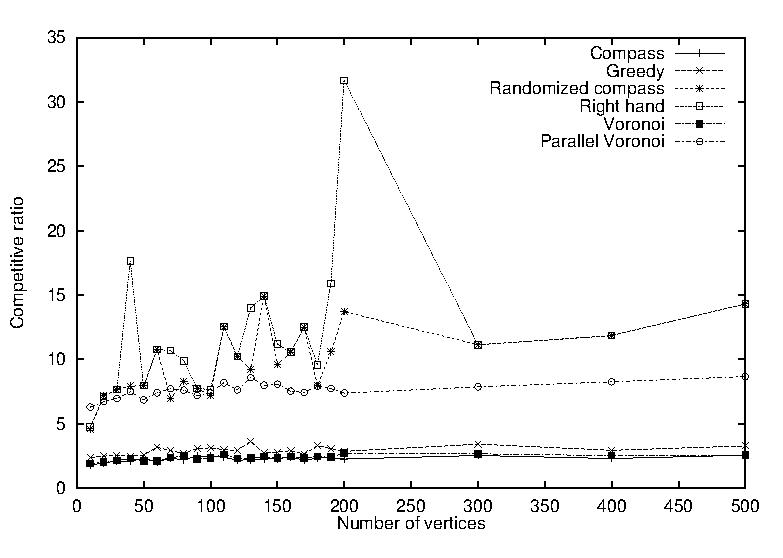
\includegraphics[height=2.5in]{delaunay}}
\caption{Empirical competitive ratios for Delaunay triangulations.}
\figlabel{delaunay}
\end{figure}
Randomized compass routing, right-hand routing, and parallel Voronoi
routing had significantly higher competitive ratios.  The results for
randomized compass routing and right-hand routing show a significant
amount of jitter.  This is due to the fact that relatively simple
configurations (see
\figref{no-competitive}.b) that can easily occur in random point
sets, result in high competitive ratios for these algorithms.  On the
other hand, parallel Voronoi routing seems much more stable, and
achieves better competitive ratios in practice than its worst case
analysis would indicate.

The most important conclusion drawn from these experiments is that there
are no simple configurations (i.e., that occur often in random point
sets) that result in extremely high competitive ratios for greedy,
compass, Voronoi, or parallel Voronoi routing in Delaunay
triangulations.  This suggests that any of these algorithms would work
well in practice.

The four simple routing algorithms of \secref{algorithms} were also
tested on Graham triangulations.  These are obtained by first sorting
the points by $x$-coordinate and then triangulating the resulting
monotone chain using a linear time algorithm for computing the convex
hull of a monotone polygonal chain \cite{ps85}.  The results are shown
in \figref{graham}. In these tests it was always the case that at
least one of the 50 independent triangulations defeated greedy
routing.  Thus, there are no results shown for greedy routing.  The
relative performance of the compass, randomized compass, and right
hand routing algorithms was the same as for Delaunay triangulations.
However, unlike the results for Delaunay triangulations, the
competitive ratio appears to be increasing linearly with the number of
vertices.

\begin{figure}
\centerline{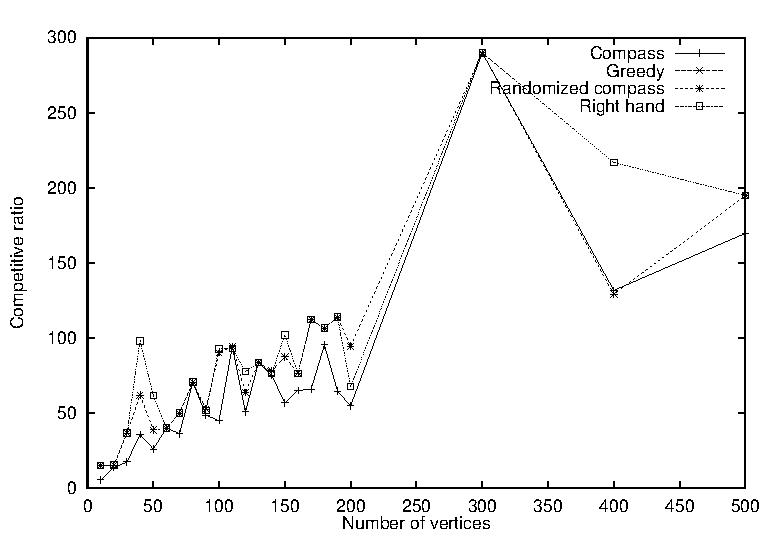
\includegraphics[height=2.5in]{graham}}
\caption{Empirical competitive ratios for Graham triangulations.}
\figlabel{graham}
\end{figure}

%%%%%%%%%%%%%%%%%%%%%%%%%%%%%%%%%%%%%%%%%%%%%%%%%%%%%%%%%%%%%%%%%%%%%
\section{Comparison with Related Work}\seclabel{related}

In this section we survey related work in the area of geometric online
routing, and compare our results with this work.  We restrict our
attention to work directly related to routing between the vertices of
geometric graphs in which the source and destination are inputs, and
do not consider routing in other geometric settings such as polygons
(c.f.\ \cite{gs97,ik95,k92}).

Keil and Gutwin \cite{kg92} give an algorithm for the construction of
a geometric graph called the $\theta$-graph for which a memoryless
routing algorithm similar to compass routing always results in a path
whose length is at most a constant (dependent only on $\theta$) times
the Euclidean distance between $\vsrc$ and $\vdest$.


Kranakis \etal\ \cite{ksu99} study compass routing, and provide a
proof that no Delaunay triangulation defeats compass routing.  The
current paper makes use of a very different proof technique to show
that compass routing works for a larger class of triangulations.  They
also describes an $O(1)$ memory routing algorithm that is not defeated
by any connected planar graph, thus proving a stronger result than
\thmref{right-hand}.

Lin and Stojmenovi\'c \cite{ls98} and Bose \etal\ \cite{bmsu99}
consider online routing in the context of \adhoc\ wireless networks
modeled by unit disk graphs.  They provide simulation results for a
variety of algorithms that measure success rates (how often a packet
never reaches its destination) as well as hop-counts of these
algorithms on unit graphs of random point sets.

Lawson's oriented walk \cite{l77} is a simple algorithm for point
location in Delaunay triangulations without preprocessing.  The
algorithm can be converted to an $O(1)$ memory routing algorithm that
is not defeated by any Delaunay triangulation.  The results of the
current paper improve on this algorithm by providing two {\em
memoryless\/} routing algorithms that are not defeated by any Delaunay
triangulation.

\comment{Generalizing results of Gold \etal\ \cite{gcr77} and
Edelsbrunner \etal\ \cite{egs86}, } De Berg \etal\ \cite{bkoo97}
describe an algorithm for enumerating all the vertices of a connected
planar subdivision using only $O(1)$ additional memory.  This
algorithm can also be viewed as an $O(1)$ memory routing algorithm.
Similarly, in any connected graph with a finite number of vertices, a
random walk will eventually visit every vertex.  Thus, random walking
can be viewed as a randomized memoryless routing algorithm that is not
defeated by any graph.  Unfortunately paths found by these techniques
will usually be much longer than the shortest path, since they are
general traversal techniques.  In contrast, the right hand routing and
randomized compass routing algorithms make use of information about
the source and destination to find more direct paths.


To the best of our knowledge, no literature currently exists on the
competitiveness of geometric routing algorithms in our abstract
setting, and our parallel Voronoi routing algorithm is the first
theoretical result in this area.  

%%%%%%%%%%%%%%%%%%%%%%%%%%%%%%%%%%%%%%%%%%%%%%%%%%%%%%%%%%%%%%%%%%%%%
\section{Conclusions}\seclabel{conclusions}

We have studied the problem of online routing in geometric graphs. Our
theoretical results show which types of graphs our algorithms are
guaranteed to work on, while our simulation results rank the
performance of the algorithms on two types of random triangulations.
These results are summarized in the \tabref{summary}.

\begin{table}
\begin{center}
\footnotesize
\begin{tabular}{|l|l|l|l|l|l|l|}\hline
Algorithm & Mem. & Rand. & Class of graphs & Rank 1 & Rank 2  
					& Competitive \\ \hline\hline
GR & None & No & Delaunay $\triangle$'s & 3 & -- & No \\
CR & None & No & Regular $\triangle$'s & 1 & 1 & No \\
RCR & None & Yes & All $\triangle$'s &      5 & 2 & No \\
RHR & $O(1)$ & No & Convex subd. & 6 & 3 & No \\
VR & $O(1)$  & No & Delaunay $\triangle$'s & 1 & -- & No\\
PVR & $O(1)$ & No & Delaunay $\triangle$'s & 4 & -- & Yes\\ \hline
\end{tabular}
\end{center}
\caption{Summary of Results}\tablabel{summary}
\end{table}

We conclude with an open problem. In \secref{algorithms} we
showed that no deterministic memoryless routing algorithm works for
every 2-connected embedded planar graph.  Can a similar argument be
made for triangulations, thus proving that randomization or memory is
necessary for a algorithm that is not defeated by any triangulation?

\section*{Acknowledgement}

The authors would like to thank \mbox{Silvia G\"otz} for reading and
commenting on an earlier version of this paper.

\bibliographystyle{siam}
\bibliography{routing}

\comment{
\version{}{
\appendix

\section{Proof of \lemref{voronoi-face}}\applabel{proofs}

\noindent{\em Proof.}[Proof (of \lemref{voronoi-face})] The following
discussion uses the notation introduced in \secref{voronoi-path}. 
\qed
}
}
\end{document}




